\section{Iteration loop}\label{iteration-loop}

In section \ref{mandelbrot-set} there was mentioned that fractals are calculated by repeating of iteration loop. The loop is terminated when there is calculated number of iterations equals to \emph{maxiter} or bailout condition is achieved.
In this section will be explained what is calculated inside the loop.

\subsection{Single formula fractals}\label{single-formula-fractals}

The simplest 3D fractals are calculated using single fractal formula which is build from many equations and conditions. These equations can be modifications of Mandelbrot Set equation or can be different mathematical equations with several conditions.

Below there are 3 examples of fractals formulas with C language code

\subsubsection{Mandelbulb Power 2}\index{Mandelbulb}
\nopagebreak

This formula is modified Mandelbrot Set equation, expanded to \nth{3} dimension. Cross section at $ z_z = 0 $ looks exactly the same as Mandelbrot Set.
\nopagebreak

\begin{tabular}{l l}
	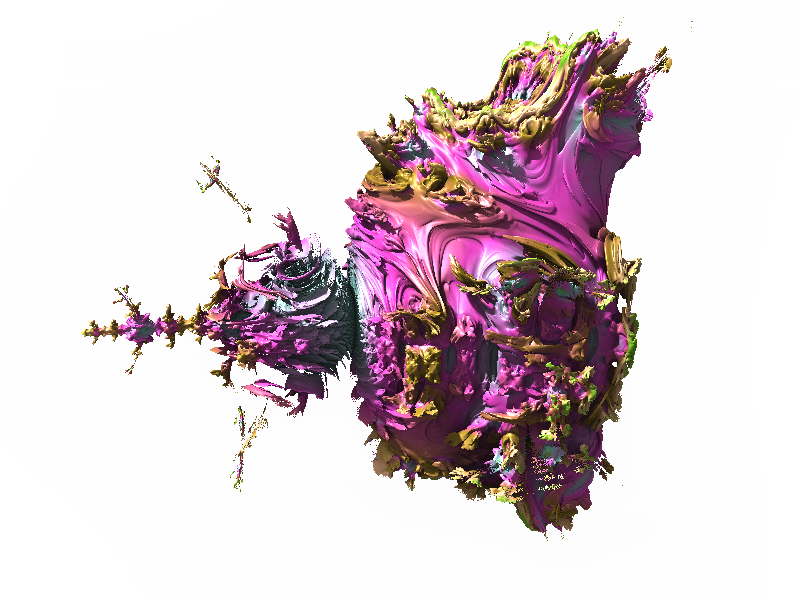
\includegraphics[width=0.3\linewidth]{img/manual/media/formula_mandelbulb_power_2}	
	& 
	\begin{minipage}[b]{0.5\linewidth}
		\begin{verbatim}[fontsize=\scriptsize]
double x2 = z.x * z.x;
double y2 = z.y * z.y;
double z2 = z.z * z.z;
double temp = 1.0 - z2 / (x2 + y2);
double newx = (x2 - y2) * temp;
double newy = 2.0 * z.x * z.y * temp;
double newz = -2.0 * z.z * sqrt(x2 + y2);
z.x = newx;
z.y = newy;
z.z = newz;
		\end{verbatim}
	\end{minipage}
\end{tabular} 

\subsubsection{Menger Sponge}\index{Menger Sponge}
\nopagebreak

This formula is Iterated Function System (IFS). It contains several transformations where some of them are conditional.
\nopagebreak

\begin{tabular}{l l}
	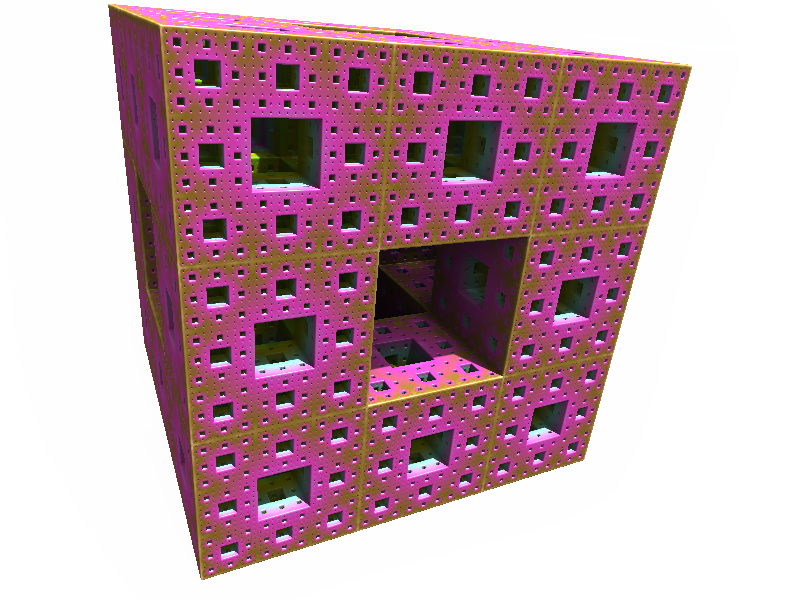
\includegraphics[width=0.3\linewidth]{img/manual/media/formula_menger_sponge.png}	
	& 
	\begin{minipage}[b]{0.5\linewidth}
		\begin{verbatim}[fontsize=\scriptsize]
z.x = fabs(z.x);
z.y = fabs(z.y);
z.z = fabs(z.z);
		
if (z.x - z.y < 0.0) swap(z.x, z.y);
if (z.x - z.z < 0.0) swap(z.x, z.z);
if (z.y - z.z < 0.0) swap(z.y, z.z);
		
z *= 3.0;
		
z.x -= 2.0;
z.y -= 2.0;
if (z.z > 1.0) z.z -= 2.0;
		\end{verbatim}
	\end{minipage}
\end{tabular} 

\subsubsection{Box Fold Bulb Pow 2}
\nopagebreak

This formula is a set of different transforms and equations. It's a good example which shows that fractal formula can be much more complicated than \emph{Mandelbrot Set}. 

First part is ``box fold''\index{transform!box fold} transform which do transformations based on box walls. Second part is ``spherical fold''\index{transform!spherical fold} which do transformations based on sphere. The end of formula is the same as \emph{Mandelbulb Power 2}. 
\nopagebreak

\begin{tabular}{l l}
	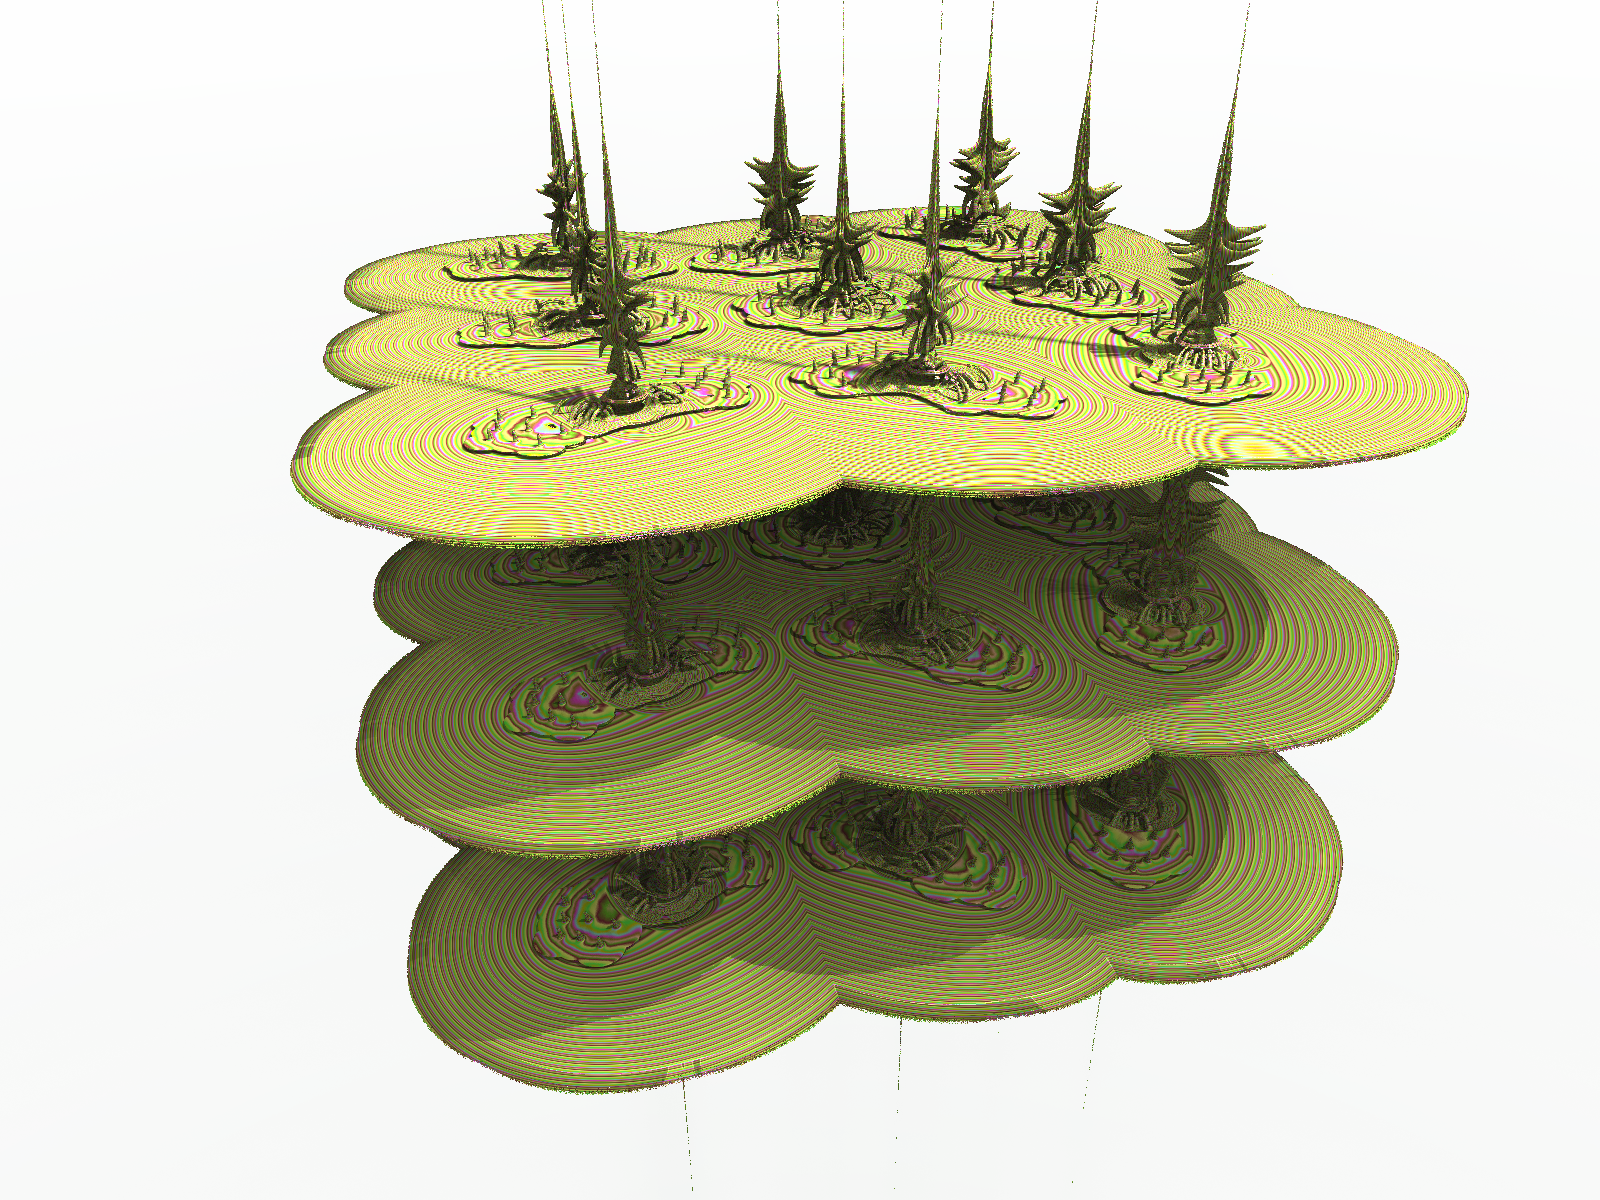
\includegraphics[width=0.3\linewidth]{img/manual/media/formula_box_fold_pwr2.png}	
	& 
	\begin{minipage}[b]{0.5\linewidth}
		\begin{verbatim}[fontsize=\scriptsize]
//box fold
if (fabs(z.x) > fractal->foldingIntPow.foldFactor)
z.x = sign(z.x) * fractal->foldingIntPow.foldFactor * 2.0 - z.x;
if (fabs(z.y) > fractal->foldingIntPow.foldFactor)
z.y = sign(z.y) * fractal->foldingIntPow.foldFactor * 2.0 - z.y;
if (fabs(z.z) > fractal->foldingIntPow.foldFactor)
z.z = sign(z.z) * fractal->foldingIntPow.foldFactor * 2.0 - z.z;

//spherical fold
double fR2_2 = 1.0;
double mR2_2 = 0.25;
double r2_2 = z.Dot(z);
double tglad_factor1_2 = fR2_2 / mR2_2;

if (r2_2 < mR2_2)
{
	z = z * tglad_factor1_2;
}
else if (r2_2 < fR2_2)
{
	double tglad_factor2_2 = fR2_2 / r2_2;
	z = z * tglad_factor2_2;
}

//Mandelbulb power 2
z = z * 2.0;
double x2 = z.x * z.x;
double y2 = z.y * z.y;
double z2 = z.z * z.z;
double temp = 1.0 - z2 / (x2 + y2);
zTemp.x = (x2 - y2) * temp;
zTemp.y = 2.0 * z.x * z.y * temp;
zTemp.z = -2.0 * z.z * sqrt(x2 + y2);
z = zTemp;
z.z *= fractal->foldingIntPow.zFactor;
		\end{verbatim}
	\end{minipage}
\end{tabular} 

\subsubsection{Processing of single formula fractals}

Single formula fractals are processed in simple way. Calculation of fractal formulas is repeated several times like it is showed on following diagrams:\nolinebreak
\nopagebreak

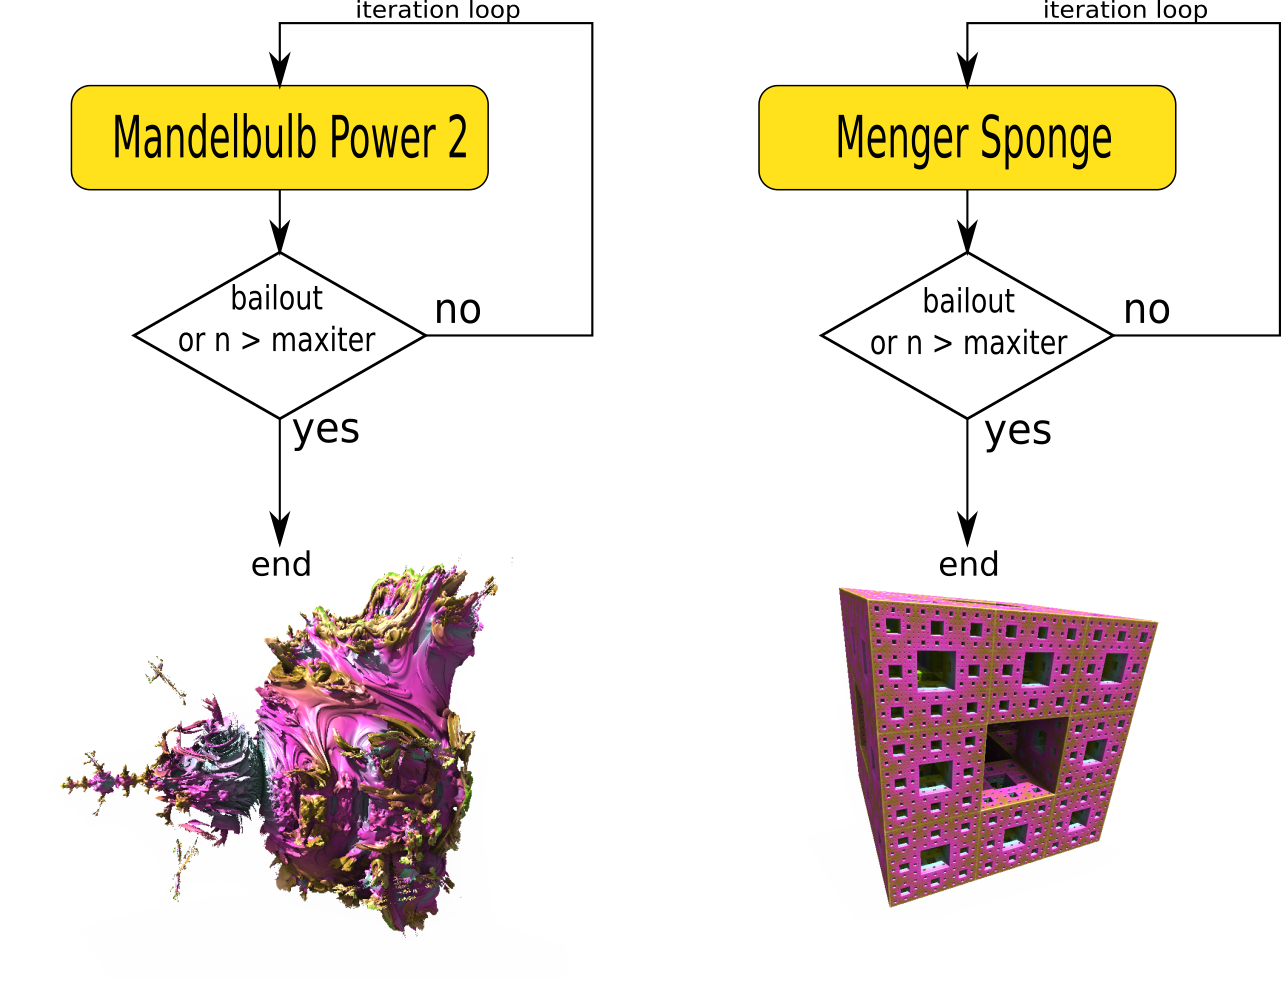
\includegraphics[width=\linewidth]{img/manual/media/iteration_loops.png}
	
When calculation of the iteration loop finished the result value of \emph{z} is used to estimate distance to fractal body and to calculate color of surface.

\subsection{Hybrid fractals}

There is possible to mix different fractal formulas by alternating them, to get new fractal shapes. That fractal are named \emph{hybrid fractals}. Mandelbulber program already have many different fractal formulas which gives opportunity to get very big variety of shapes. But using hybrid fractals increases possibilities a lot. 

\subsubsection{Processing of hybrid fractals}

%TODO write text about hybrid fractals

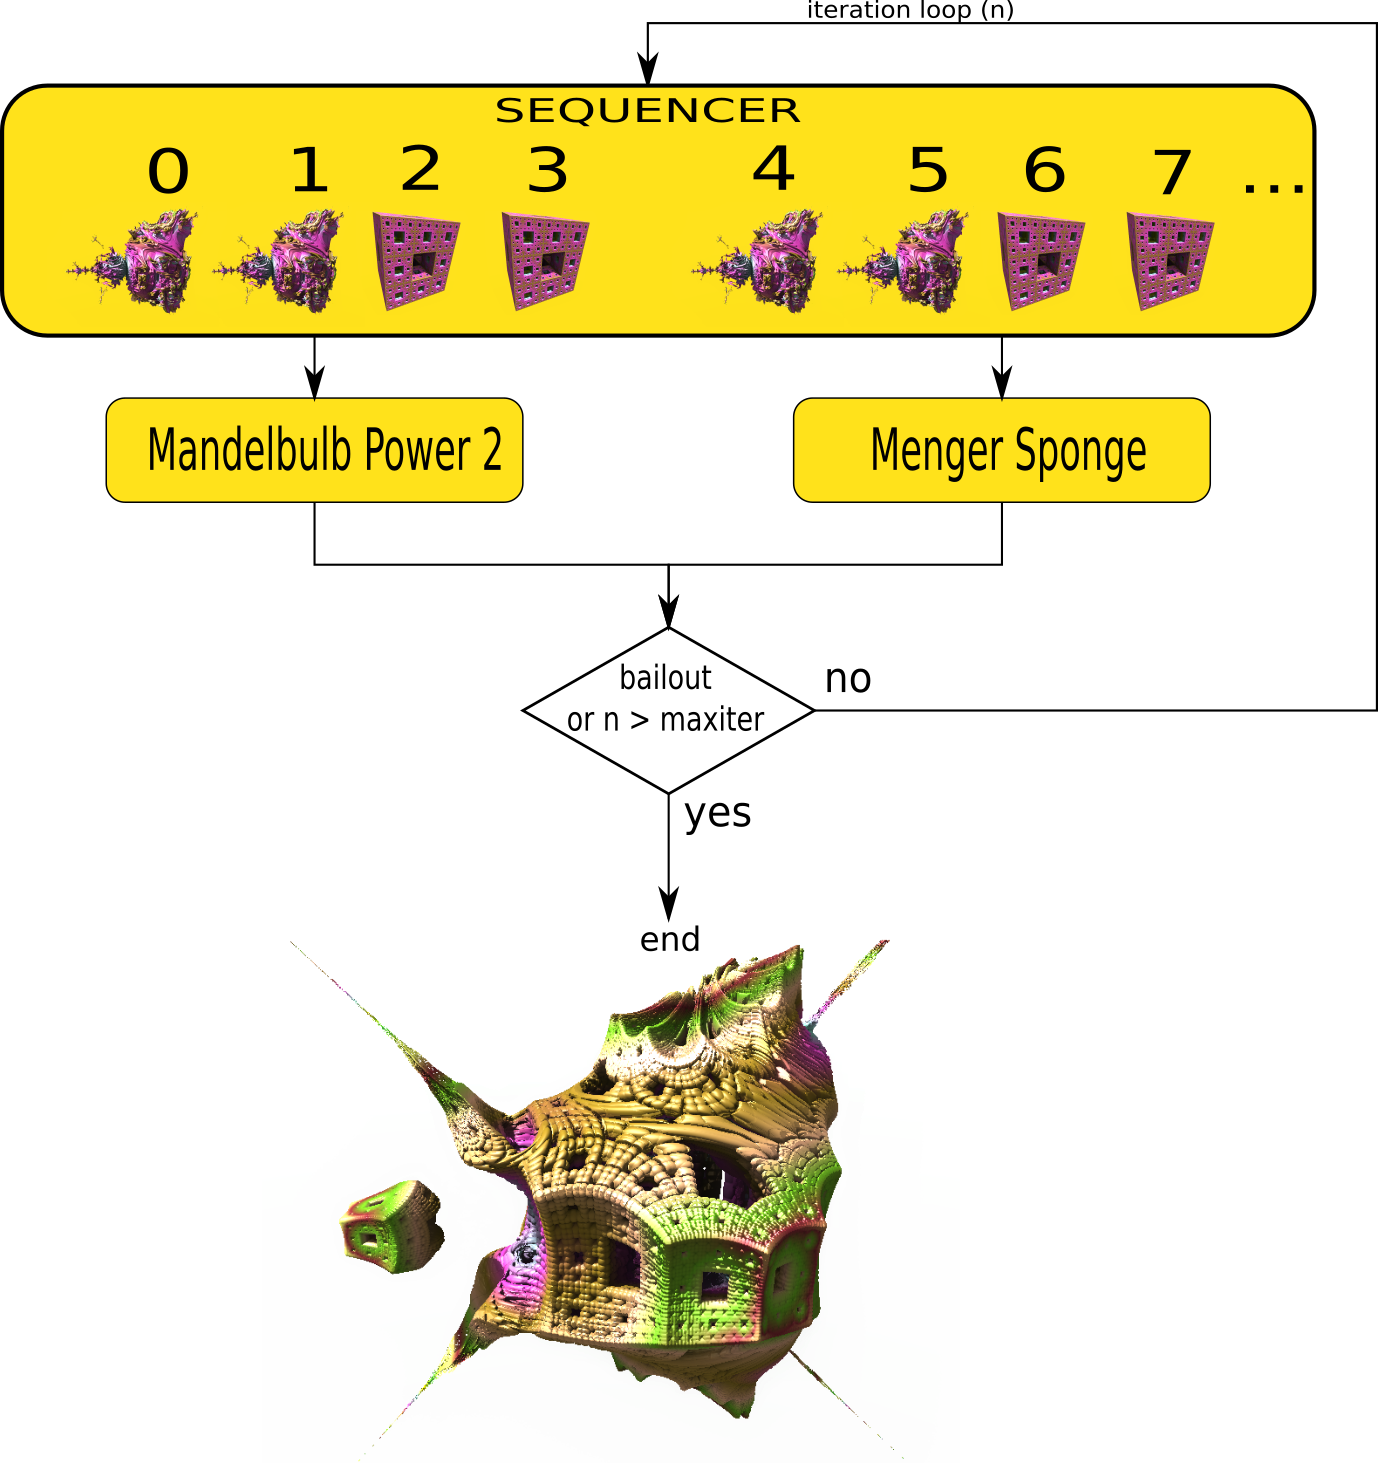
\includegraphics[width=\linewidth]{img/manual/media/iteration_loop_hybrid.png}

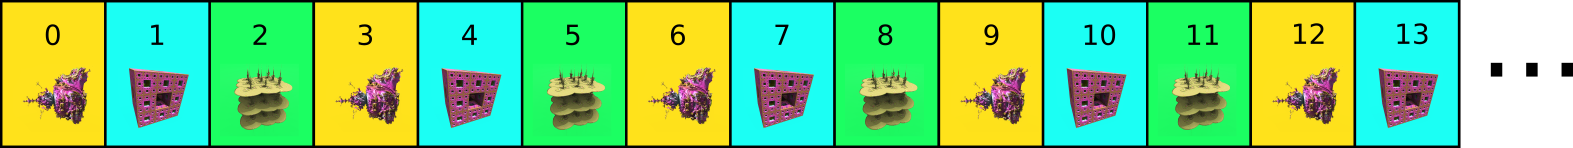
\includegraphics[width=\linewidth]{img/manual/media/iteration_loop_hybrid_sequence_1.png}

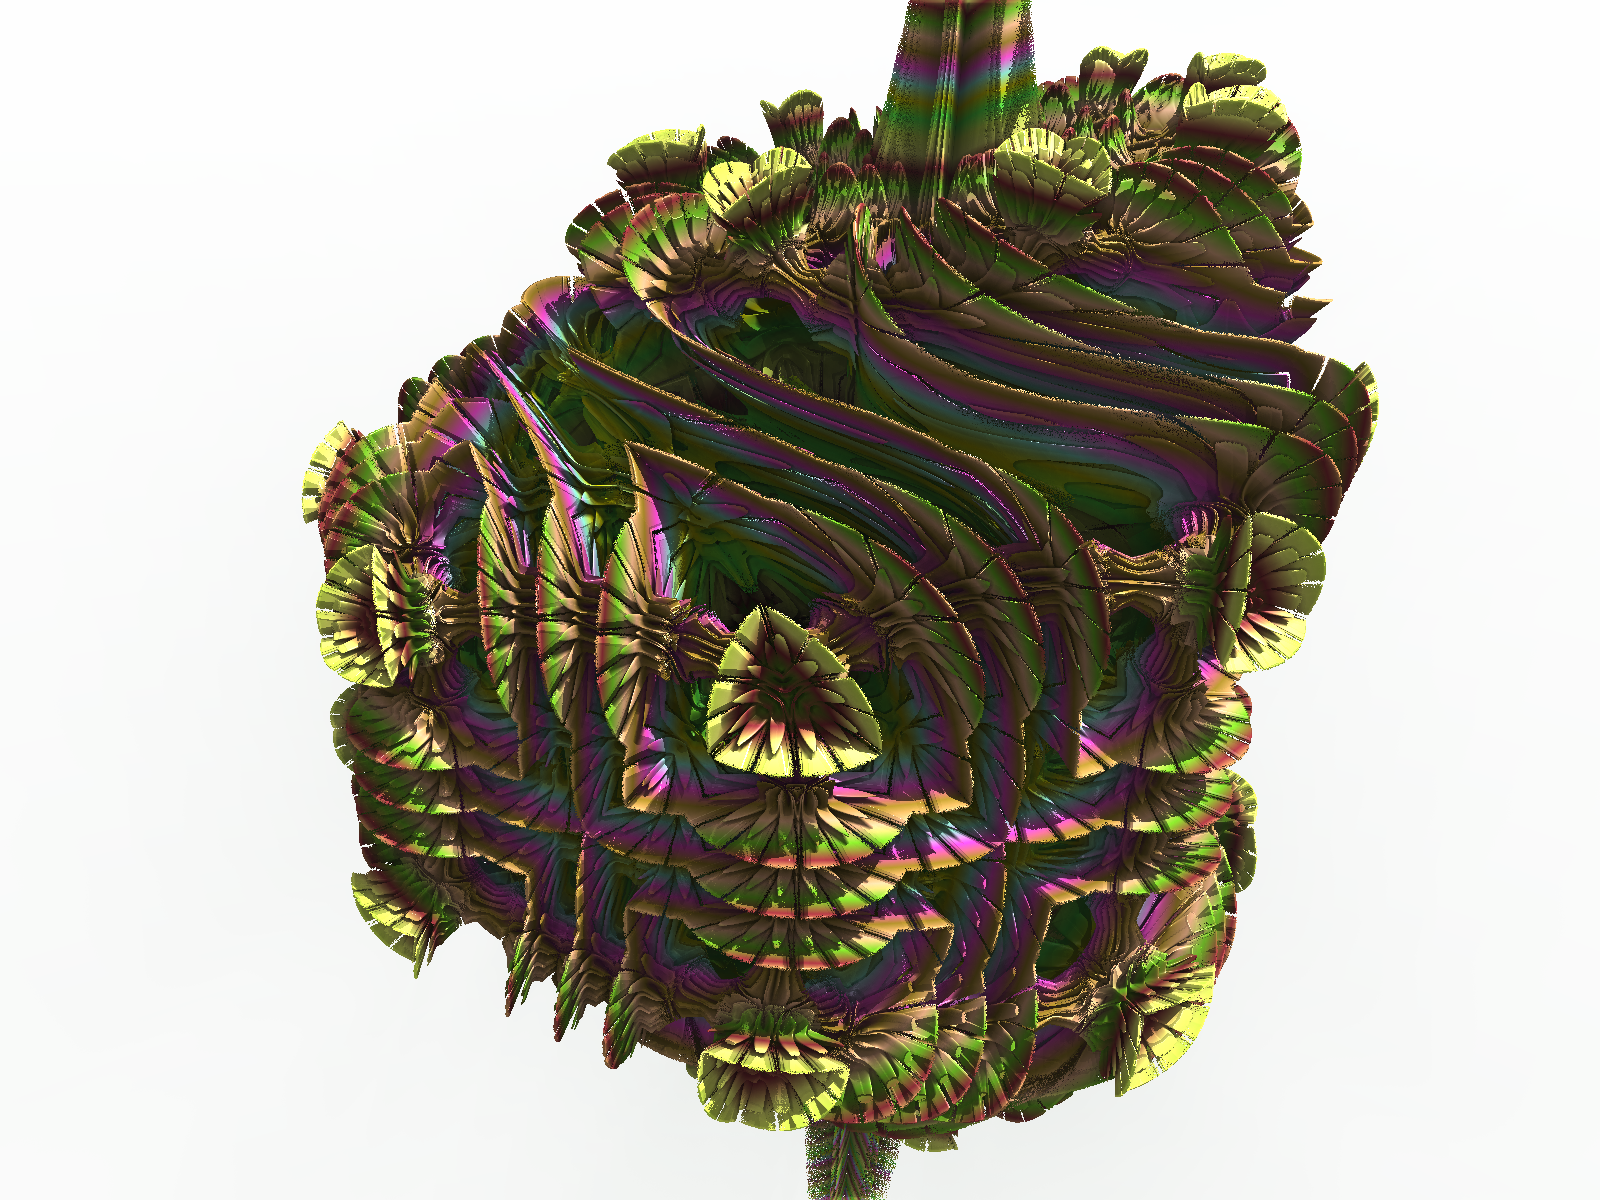
\includegraphics[width=0.7\linewidth]{img/manual/media/hybrid_sequence_example_1.png}

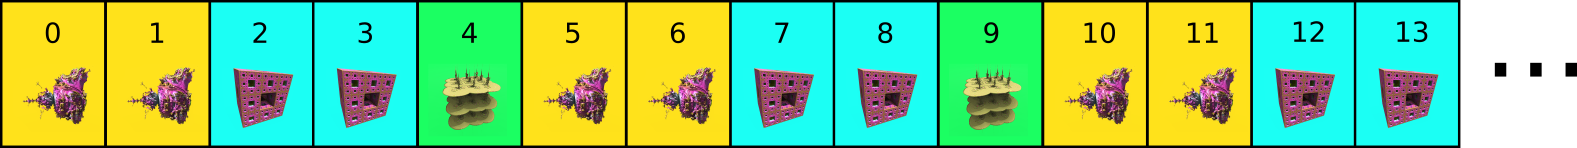
\includegraphics[width=\linewidth]{img/manual/media/iteration_loop_hybrid_sequence_2.png}

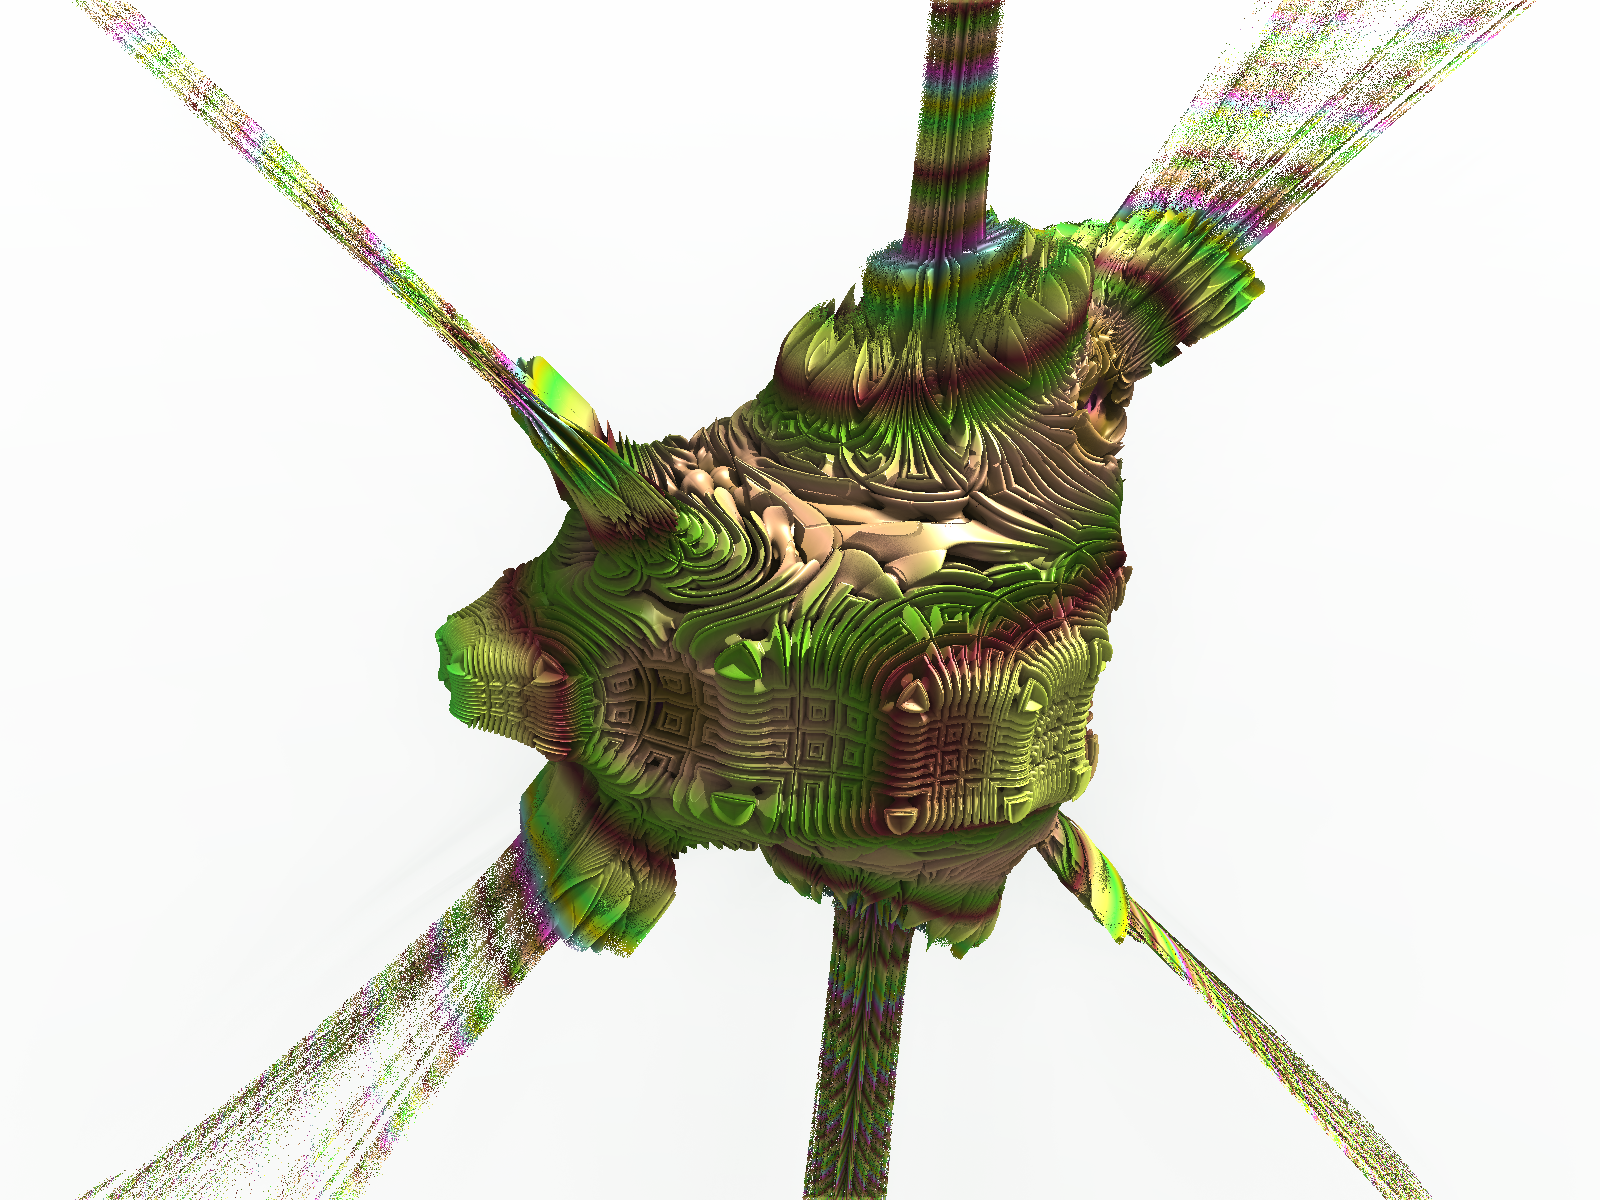
\includegraphics[width=0.7\linewidth]{img/manual/media/hybrid_sequence_example_2.png}

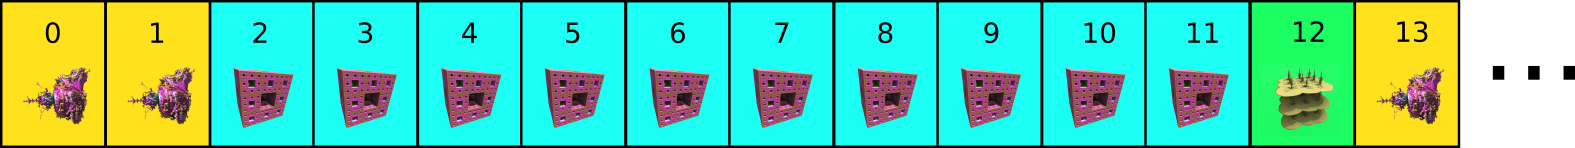
\includegraphics[width=\linewidth]{img/manual/media/iteration_loop_hybrid_sequence_3.png}

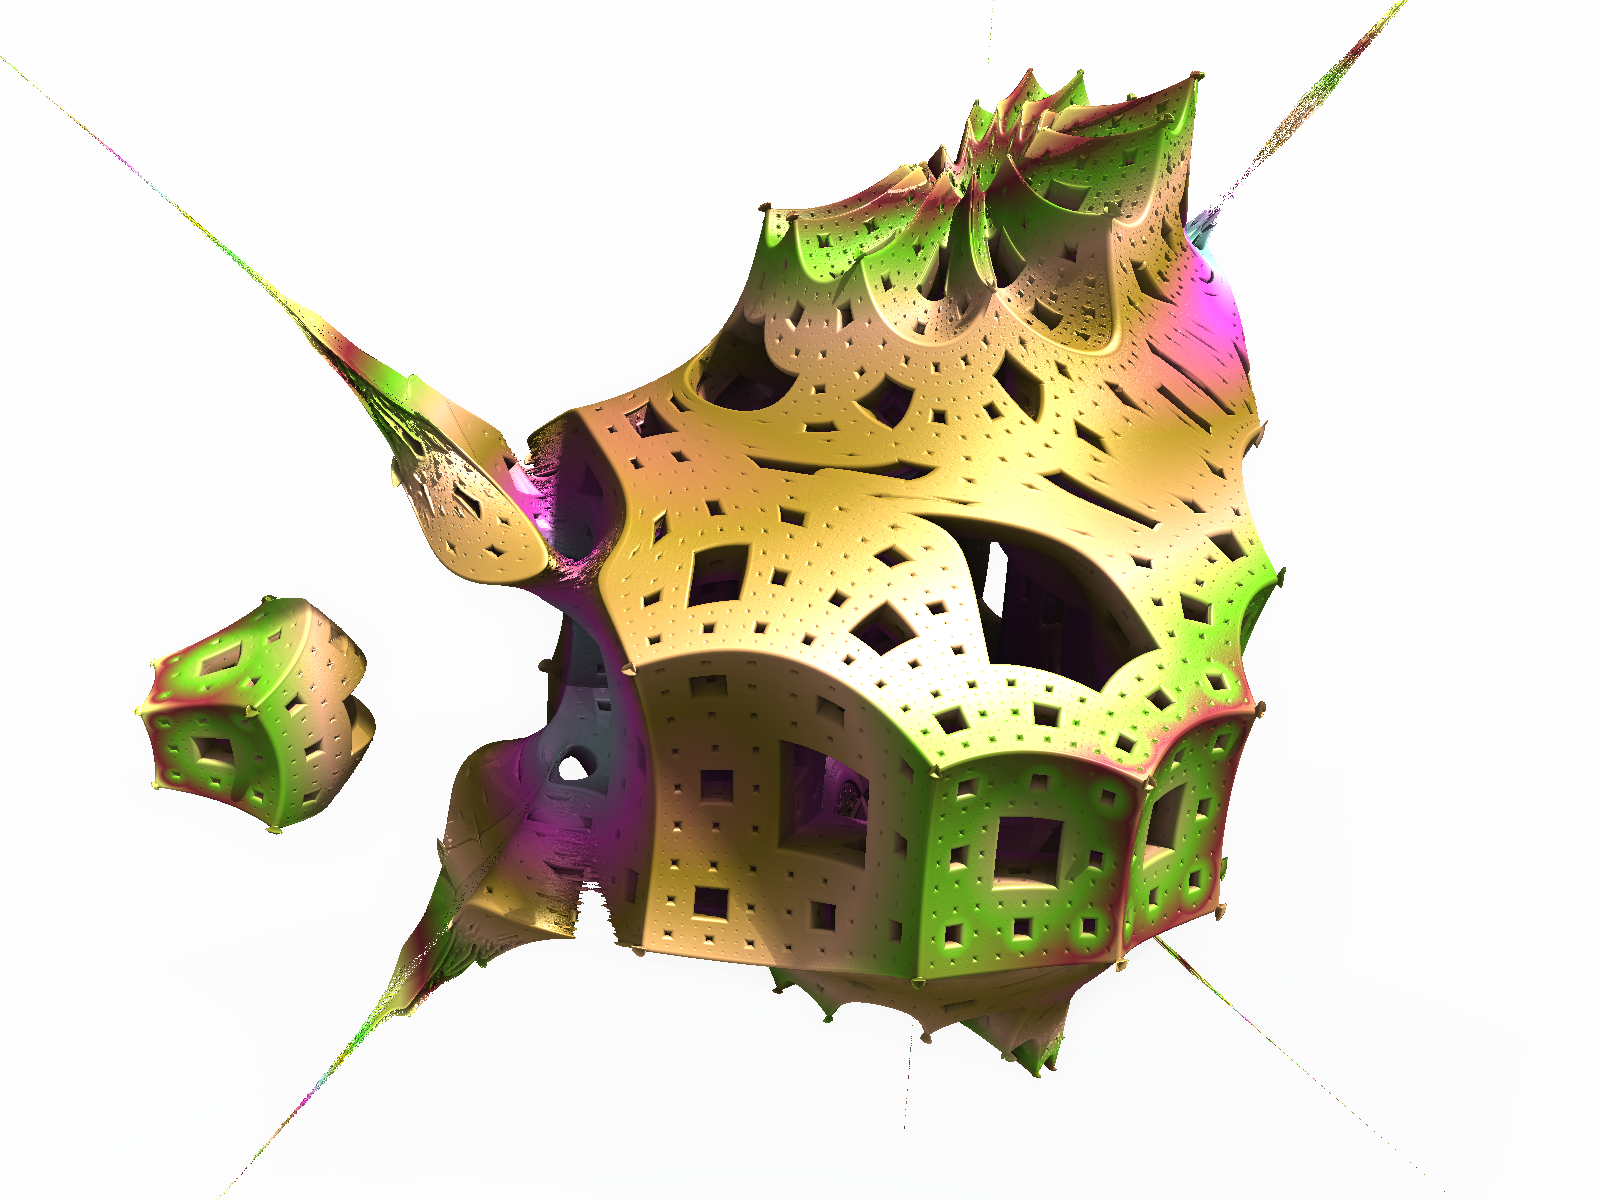
\includegraphics[width=0.7\linewidth]{img/manual/media/hybrid_sequence_example_3.png}

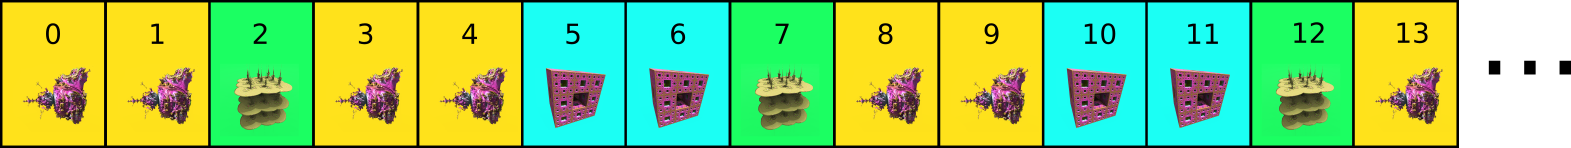
\includegraphics[width=\linewidth]{img/manual/media/iteration_loop_hybrid_sequence_4.png}

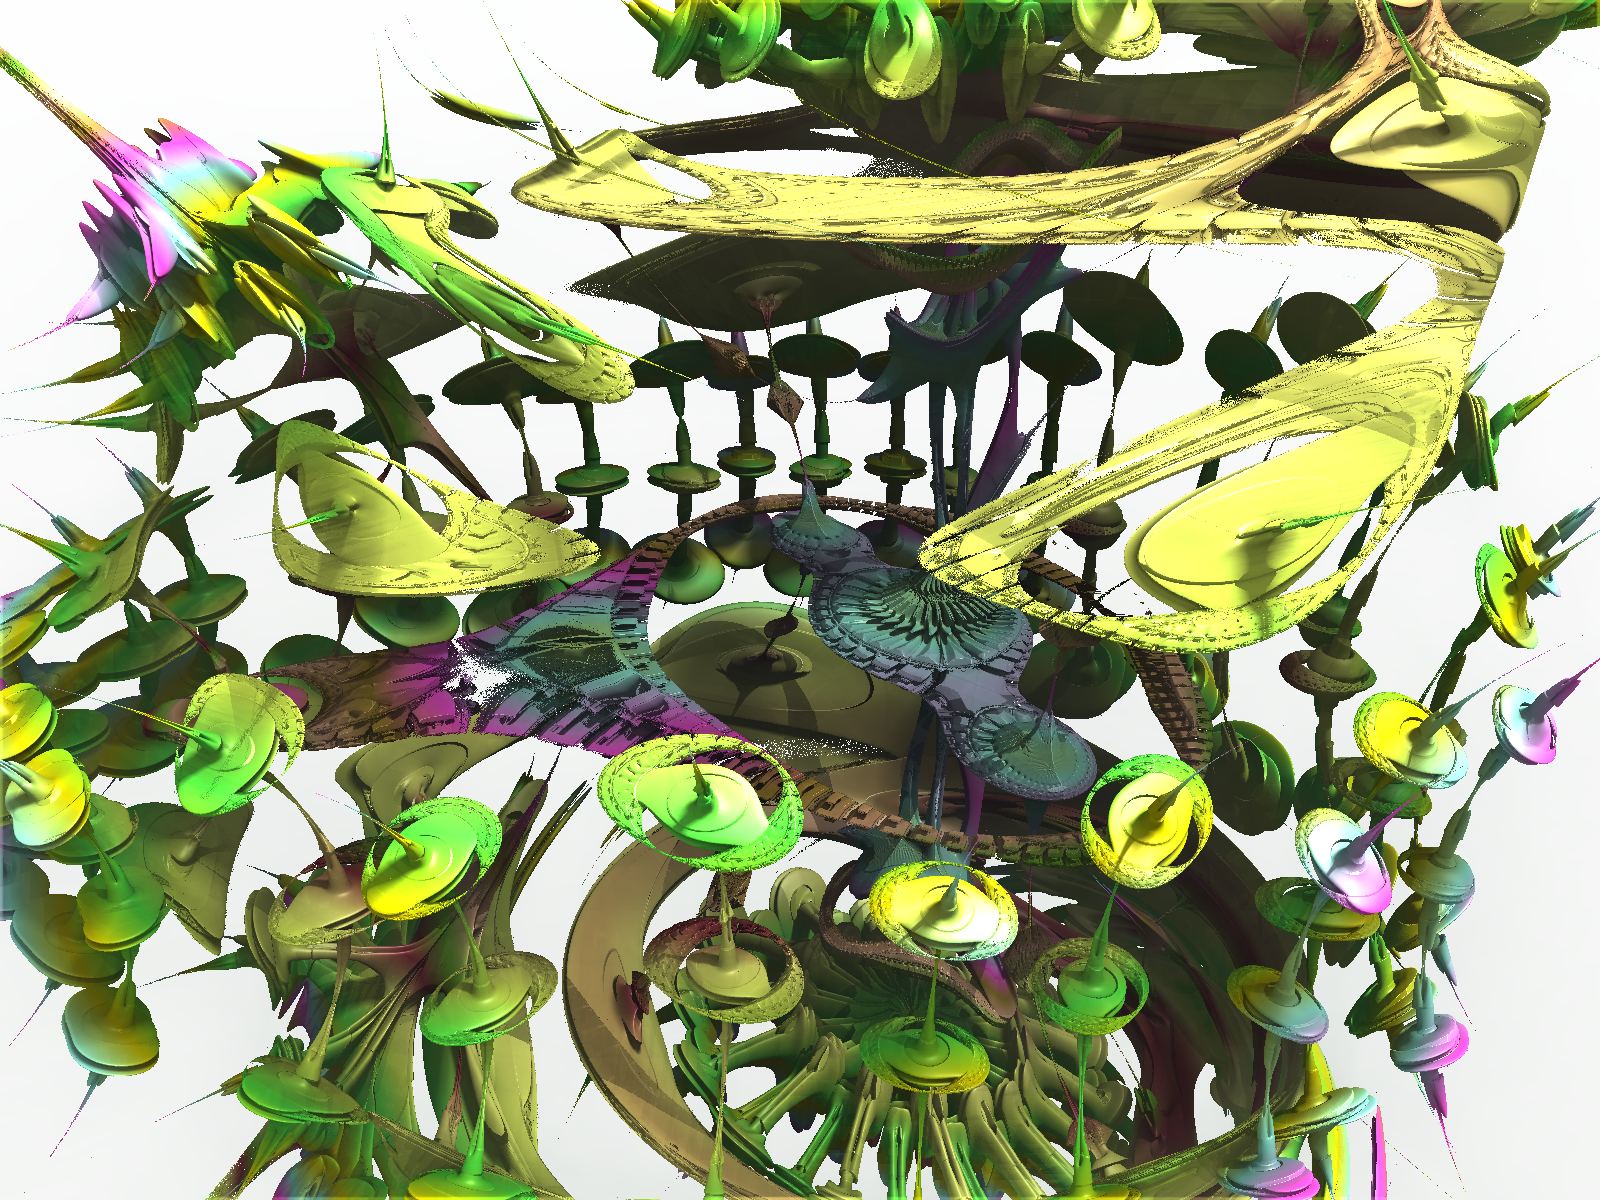
\includegraphics[width=0.7\linewidth]{img/manual/media/hybrid_sequence_example_4.png}

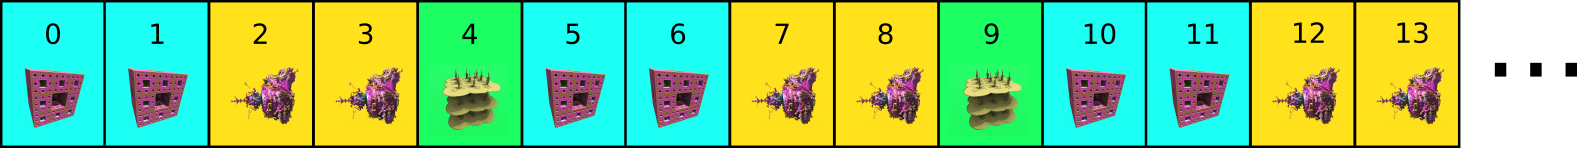
\includegraphics[width=\linewidth]{img/manual/media/iteration_loop_hybrid_sequence_5.png}

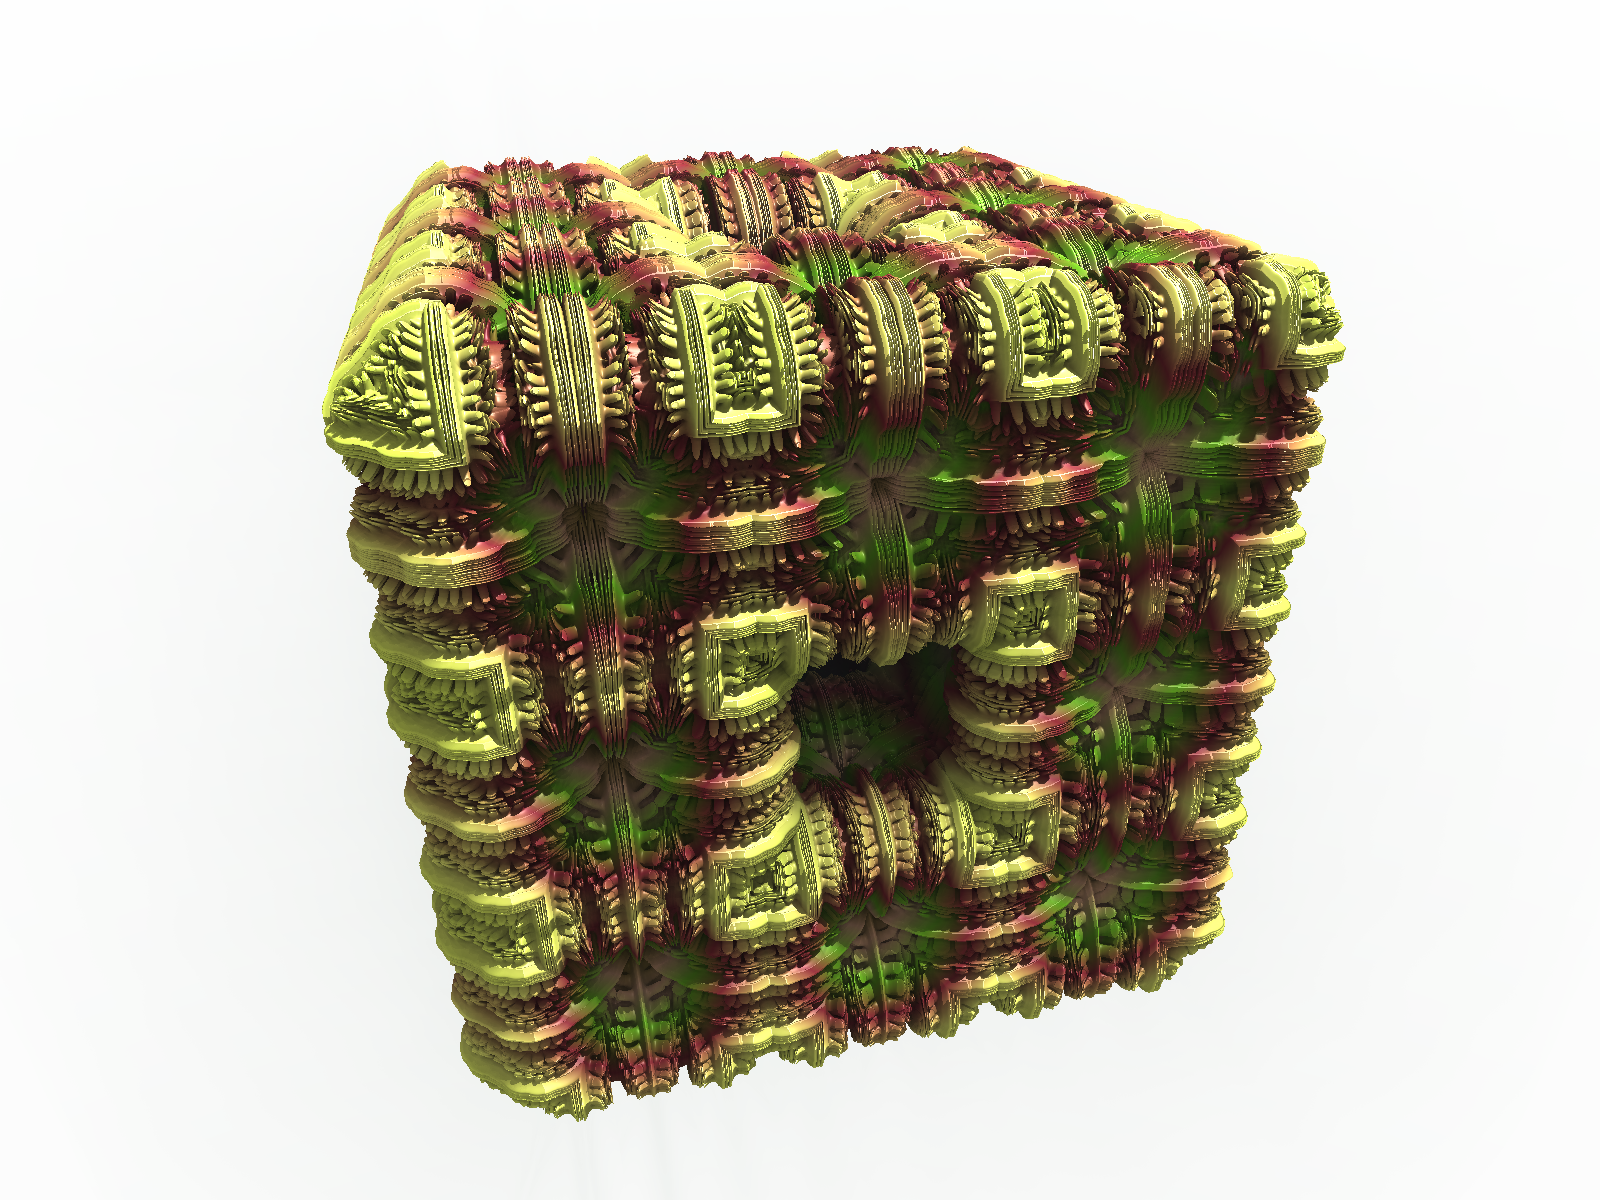
\includegraphics[width=0.7\linewidth]{img/manual/media/hybrid_sequence_example_5.png}
